\caulc
\Opensolutionfile{ans}[ans/ansTN-Dung]
%%%=============EX_1=============%%%
\begin{ex}%[2H2H2-4]%[TDMT09]%[Bồ Văn Hậu]
	Trong không gian $Oxyz$, độ dài của tổng hai vectơ $\overrightarrow{u}=(3;1;-1)$, $\overrightarrow{v}=(1;3;3)$ là
	\choice
	{$(4;2;2)$}
	{\True $6$}
	{$10$}
	{$5$}
	\loigiai{
		Ta có $\overrightarrow{u}+\overrightarrow{v}=(4;4;2)$.\\
		Suy ra $\left|\overrightarrow{u}+\overrightarrow{v}\right|=\sqrt{4^2+4^2+2^2}=6$.
	}
\end{ex}
%%%=============================%%%

%%%=============EX_2=============%%%
\begin{ex}%[1D2N3-3]%[TDMT09]%[Đình Nguyên]
	Cho cấp số nhân $(u_n)$ có $u_1 = 1$ và $u_4 = 27$. Công bội của $(u_n)$ bằng
	\choice
	{$1$}
	{$2$}
	{\True $3$}
	{$3\sqrt{3}$}
	\loigiai{
		Ta có $u_4 = u_1 \cdot q^3 \Leftrightarrow 27 = 1 \cdot q^3 \Leftrightarrow q = 3$.
	}
\end{ex}
%%%=============================%%%

%%%=============EX_3=============%%%
\begin{ex}%[TDM21]%[2D1N2-2]
	Số điểm cực trị của hàm số $f(x) = x^4 - 2x^2 - 2026$ là
	\choice
	{\True $3$}
	{$2$}
	{$1$}
	{$0$}
	\loigiai{
		\textbf{Cách 1:}\\
		Tập xác định $\mathscr{D} = \mathbb{R}$.\\
		Đạo hàm $f'(x) = 4x^3 - 4x$.\\
		Ta có $f'(x) = 0 \Leftrightarrow 4x^3 - 4x = 0 \Leftrightarrow \hoac{&x = 0 \\ &x = 1 \\ &x = -1.}$\\
		Phương trình $f'(x) = 0$ có $3$ nghiệm đơn phân biệt nên hàm số đã cho có $3$ điểm cực trị.\\
		\textbf{Cách 2:}\\
		Hàm số bậc bốn trùng phương $f(x) = ax^4 + bx^2 + c$ có các hệ số $a = 1$, $b = -2$.\\
		Vì $a \cdot b = 1 \cdot (-2) = -2 < 0$ nên hàm số đã cho có $3$ điểm cực trị.
	}
\end{ex}
%%%=============================%%%

%%%=============EX_4=============%%%
\begin{ex}%[2H2N2-3]%[TDMT09]%[Mui Doan]
	Trong không gian $Oxyz$, cho hai điểm $A(1;2;-2)$, $B(3;4;1)$. Hãy xác định tọa độ của vectơ $\overrightarrow{BA}$.
	\choice
	{$(2;2;3)$}
	{\True $(-2;-2;-3)$}
	{$(4;6;-1)$}
	{$(1;3;0)$}
	\loigiai{
		Ta có $	\overrightarrow{BA} = (1-3;2-4;-2-1)= (-2;-2;-3)$.
	}
\end{ex}
%%%=============================%%%

%%%=============EX_5=============%%%
\begin{ex}%[2D1N1-2]%[TDMT09]%[Nguyễn Trí Minh Tuấn]
	\immini[thm]{Cho đồ thị hàm số $y=f'(x)$ như hình vẽ. Hàm số $f(x)$ nghịch biến trên khoảng
		\choice
		{\True $(-\infty;-4)$}
		{$(0;7)$}
		{$(-\infty;0)$}
		{$(7;+\infty)$}
	}{
		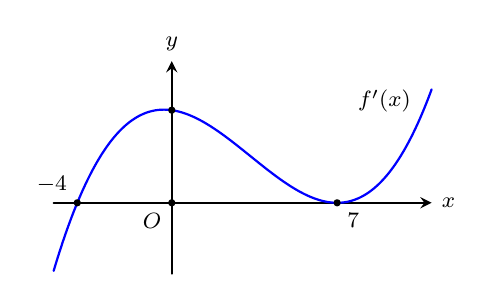
\begin{tikzpicture}[scale=0.3, line cap=round, line join=round, >=stealth, font=\footnotesize, thick]
			\draw[->] (-5,0)--(11,0) node[right] {$x$};
			\draw[->] (0,-3)--(0,6) node[above] {$y$};
			\draw[blue, smooth, domain=-5:11, samples=200] plot (\x,{0.02*(\x+4)*(\x-7)*(\x-7)});
			\filldraw (-4,0) circle (3pt) node[above left] {$-4$}
			(7,0) circle (3pt) node[below right] {$7$}
			(0,0) circle (3pt) node[below left] {$O$}
			(0,{0.02*(0+4)*(0-7)*(0-7)}) circle (3pt);
			\node at (9,4.3) {$f'(x)$};
		\end{tikzpicture}
	}
	\loigiai{
		Dựa vào đồ thị $y=f'(x)$, ta thấy $f'(x)<0$ khi $x<-4$.\\
		Do đó, hàm số $f(x)$ nghịch biến trên khoảng $(-\infty;-4)$.
	}
\end{ex}
%%%=============================%%%

%%%=============EX_6=============%%%
\begin{ex}%[TDMT9]%[1H8N7-1]%[Huỳnh Quốc Đạt]
	Cho khối chóp có diện tích đáy bằng $3$ và chiều cao bằng $2$. Thể tích của khối chóp này bằng
	\choice
	{$6$}
	{$5$}
	{$18$}
	{\True $2$}
	\loigiai{
		Thể tích khối chóp $V=\dfrac{1}{3}Sh=\dfrac{1}{3}\cdot 3\cdot 2 = 2$.
	}
\end{ex}
%%%=============================%%%

%%%=============EX_7=============%%%
\begin{ex}%[2D1H4-1]%[TDMT09]%[Chu Ha]
	Hỏi đồ thị hàm số $y=\dfrac{x^2-4x+3}{x^3-x}$ có tất cả bao nhiêu đường tiệm cận đứng?
	\choice
	{$0$}
	{$1$}
	{\True $2$}
	{$3$}
	\loigiai{
		Tập xác định $\mathscr{D}=\mathbb{R}\setminus \{-1;0;1\}$.\\
		Ta có
		$y=\dfrac{(x-1)(x-3)}{x(x-1)(x+1)}=\dfrac{x-3}{x(x+1)}$.\\
		Xét các giới hạn
		\begin{itemize}
			\item $\displaystyle \lim\limits_{x\to 0^\pm}\dfrac{x-3}{x(x+1)}=\mp\infty$ nên $x=0$ là tiệm cận đứng.
			\item $\displaystyle \lim\limits_{x\to -1^\pm}\dfrac{x-3}{x(x+1)}=\pm\infty$ nên $x=-1$ là tiệm cận đứng.
			\item Tại $x=1$ ta có $\displaystyle \lim\limits_{x\to 1}\dfrac{x^2-4x+3}{x^3-x}=\lim\limits_{x\to 1}\dfrac{x-3}{x(x+1)}=-1$ nên $x=1$ không là tiệm cận đứng.
		\end{itemize}
		Vậy đồ thị hàm số có $2$ đường tiệm cận đứng.
	}
\end{ex}
%%%=============================%%%

%%%=============EX_8=============%%%
\begin{ex}%[0D3H2-2]%[TDMT09]%[Nguyễn Tấn Linh]
	Giá trị nhỏ nhất của hàm số $y=(x^2+1)^2+2$ là
	\choice
	{\True $3$}
	{$2$}
	{$1$}
	{$4$}
	\loigiai{
		Ta có $x^2 \ge 0$, $\forall x \in \mathbb{R} \Rightarrow x^2+1 \ge 1 \Rightarrow (x^2+1)^2 \ge 1$.\\
		Khi đó $y=(x^2+1)^2+2 \ge 1+2=3$.\\
		Dấu đẳng thức xảy ra khi và chỉ khi $x=0$.\\
		Vậy giá trị nhỏ nhất của hàm số bằng $3$.
	}
\end{ex}
%%%=============================%%%

%%%=============EX_9=============%%%
\begin{ex}%[2D1H4-3]%[TDMT09]%[Lê Phúc]
	Tâm đối xứng của đồ thị hàm số $y=\dfrac{x^2-6x+6}{x-1}$ là
	\choice
	{$M(1;4)$}
	{$N(5;1)$}
	{$P(0;-6)$}
	{\True $Q(1;-4)$}
	\loigiai{
		Ta có $y=\dfrac{x^2-6x+6}{x-1}=x-5+\dfrac{1}{x-1}$.\\
		Ta có $\lim\limits_{x\to1^+}y=\lim\limits_{x\to1^+}\dfrac{x^2-6x+6}{x-1}=+\infty$.\\
		Suy ra $x=1$ là tiệm cận đứng của đồ thị hàm số.\\
		Ta lại có $\lim\limits_{x\to+\infty}\left[y-(x-5)\right]=\lim\limits_{x\to+\infty}\left(\dfrac{1}{x-1}\right)=0$.\\
		Suy ra $y=x-5$ là tiệm cận xiên của đồ thị hàm số.\\
		Do tâm đối xứng là giao điểm của hai đường tiệm cận nên tọa độ tâm đối xứng thỏa mãn hệ phương trình
		\[\heva{&x=1\\&y=x-5}\Leftrightarrow\heva{&x=1\\&y=-4.}\]
		Vậy tâm đối xứng của đồ thị hàm số là $Q(1;-4)$.
	}
\end{ex}
%%%=============================%%%

\begin{ex}
	\sochc{2}
	Cho hình hộp $ABCD.A'B'C'D'$ có tất cả các cạnh đều bằng $6$. Biết rằng $\widehat{BAD} = 60^\circ$, $\widehat{BAA'} = 90^\circ$, $\widehat{DAA'} = 60^\circ$ 
	\begin{chc}%[2H2H1-3]%[TDMTD09]%[Phạm Hải Dương]
		Đáp án nhận xét \textbf{sai} là
		\choice
		{$\overrightarrow{AB} \cdot \overrightarrow{AD} = 18$}
		{$\overrightarrow{AB} \cdot \overrightarrow{AA'} = 0$}
		{\True $\overrightarrow{AD} \cdot \overrightarrow{AA'} = -18$}
		{$\overrightarrow{AB} \cdot \overrightarrow{CC'} = 0$}
		\loigiai{
			Dựa vào giả thiết các cạnh bằng $6$ và các góc tại đỉnh $A$, ta tính tích vô hướng của các cặp vectơ:
			\begin{itemize}
				\item $\overrightarrow{AB} \cdot \overrightarrow{AD} = \left|\overrightarrow{AB}\right| \cdot \left|\overrightarrow{AD}\right| \cdot \cos \widehat{BAD} = 6 \cdot 6 \cdot \cos 60^\circ = 36 \cdot \dfrac{1}{2} = 18$.
				\item $\overrightarrow{AB} \cdot \overrightarrow{AA'} = \left|\overrightarrow{AB}\right| \cdot \left|\overrightarrow{AA'}\right| \cdot \cos \widehat{BAA'} = 6 \cdot 6 \cdot \cos 90^\circ = 6 \cdot 6 \cdot 0 = 0$.
				\item $\overrightarrow{AD} \cdot \overrightarrow{AA'} = \left|\overrightarrow{AD}\right| \cdot \left|\overrightarrow{AA'}\right| \cdot \cos \widehat{DAA'} = 6 \cdot 6 \cdot \cos 60^\circ = 36 \cdot \dfrac{1}{2} = 18$.
				\item $\overrightarrow{AB} \cdot \overrightarrow{CC'} = \overrightarrow{AB} \cdot \overrightarrow{AA'} = 0$ (do $\overrightarrow{CC'} = \overrightarrow{AA'}$).
			\end{itemize}
		}
	\end{chc}
	%%%=============================%%%
	
	%%%=============EX_11=============%%%
	\begin{chc}%[2H2H1-3]%[TDMT09]%[Huỳnh Trí Thiện]
		Độ dài đường chéo $AC'$ bằng 
		\choice
		{\True $6\sqrt{5}$}
		{$12$}
		{$6\sqrt{6}$}
		{$12$}
		\loigiai{
			Ta có $\overrightarrow{AC'} = \overrightarrow{AB} + \overrightarrow{AD} + \overrightarrow{AA'}$.\\
			Suy ra
			\allowdisplaybreaks
			\begin{align*}
				AC'^2 = \overrightarrow{AC'}^2 &= \left(\overrightarrow{AB} + \overrightarrow{AD} + \overrightarrow{AA'}\right)^2 \\
				&= AB^2 + AD^2 + AA'^2 + 2\overrightarrow{AB}\cdot\overrightarrow{AD} + 2\overrightarrow{AB}\cdot\overrightarrow{AA'} + 2\overrightarrow{AD}\cdot\overrightarrow{AA'} \\
				&= 6^2 + 6^2 + 6^2 + 2 \cdot 6 \cdot 6 \cdot \cos\left(\widehat{BAD}\right) + 2 \cdot 6 \cdot 6 \cdot \cos\left(\widehat{BAA'}\right) + 2 \cdot 6 \cdot 6 \cdot \cos\left(\widehat{DAA'}\right) \\
				&= 108 + 72\cdot\cos 60^\circ + 72\cdot\cos 90^\circ + 72\cdot\cos 60^\circ \\
				&= 108 + 36 + 36 = 180.
			\end{align*}
			Vậy $AC' = \sqrt{180} = 6\sqrt{5}$.
		}
	\end{chc}
	%%%=============================%%%
\end{ex}

%%%=============EX_12=============%%%
\begin{ex}%[2D1V4-1]%[TDMT09]%[Nguyễn Sơn Thành]
	Cho bảng biến thiên của hàm số $f(x)$ như hình vẽ bên dưới. Tổng số đường tiệm cận đứng và tiệm cận ngang của đồ thị hàm số $y = \dfrac{1}{2 - \sqrt{f(x)}}$ là
	\begin{center}
		
\begin{tikzpicture}
			\tkzTabInit[lgt=1.2,espcl=3,nocadre=false]
			{$x$/0.7,$f(x)$/2}
			{$-\infty$,$-2$,$3$,$6$,$+\infty$}
			\tkzTabVar{+/$-1$, -/$-3$, +/$8$, -/$-4$, +/$0$}
		\end{tikzpicture}
	\end{center}
	\choice
	{$3$}
	{$1$}
	{$4$}
	{\True $2$}
	\loigiai{
		\begin{enumerate}
			\item Tìm đường tiệm cận ngang
			\begin{itemize}
				\item Khi $x \to -\infty$, ta có $f(x) \to -1 < 0$ nên $\sqrt{f(x)}$ không xác định.
				\item Khi $x \to +\infty$, dựa vào bảng biến thiên ta thấy $f(x)$ tăng từ $-4$ đến $0$, tức là $f(x) < 0$. Do đó $\sqrt{f(x)}$ cũng không xác định.
			\end{itemize}
			Vậy đồ thị không có đường tiệm cận ngang.
			\item Tìm đường tiệm cận đứng
			\begin{itemize}
				\item Tiệm cận đứng xảy ra tại các giá trị $x$ làm cho mẫu số bằng $0$ và thỏa mãn điều kiện xác định ($f(x) \ge 0$).
				\item Ta có $2 - \sqrt{f(x)} = 0 \Leftrightarrow \sqrt{f(x)} = 2 \Leftrightarrow f(x) = 4$.
				\item Dựa vào bảng biến thiên, đường thẳng $y=4$ cắt đồ thị tại $2$ điểm phân biệt (một điểm thuộc khoảng $(-2;3)$ vì $-3 < 4 < 8$, một điểm thuộc khoảng $(3;6)$ vì $-4 < 4 < 8$). Tại các điểm này $f(x)=4 > 0$ nên thỏa mãn điều kiện.
				\item Suy ra số đường tiệm cận đứng của đồ thị hàm số là $2$.
			\end{itemize}
		\end{enumerate}
		Vậy tổng số đường tiệm cận đứng và tiệm cận ngang là $0 + 2 = 2$.
	}
\end{ex}
%%%=============================%%%
\Closesolutionfile{ans}

\cauds
\Opensolutionfile{ans}[ans/ansTN-DungSai]
%%%=============EX_13=============%%%
\begin{ex}%[2H2V2-5]
	Trong không gian $Oxyz$, cho ba điểm $A(2;0;1)$, $B(0;1;1)$, $C(2;2;3)$.
	\choiceTF[t]
	{\True $AB = \sqrt{5}$}
	{\True $\cos\left(\overrightarrow{AB}, \overrightarrow{AC}\right) = \dfrac{1}{\sqrt{10}}$}
	{Bán kính đường tròn ngoại tiếp tam giác $ABC$ là $R = \sqrt{10}$}
	{\True Gọi $M$ là điểm thay đổi trong không gian $Oxyz$. Khi đó giá trị nhỏ nhất của biểu thức $OM + MA + MB + MC$ bằng $6{,}4$ \textit{(làm tròn kết quả đến hàng phần mười)}}
	\loigiai{
		Ta có $\overrightarrow{AB} = (-2;1;0)$, $\overrightarrow{AC} = (0;2;2)$ và $\overrightarrow{BC} = (2;1;2)$.\\
		Suy ra $AB = \sqrt{4 + 1 + 0} = \sqrt{5}$, $AC = \sqrt{0 + 4 + 4} = 2\sqrt{2}$, $BC = \sqrt{4 + 1 + 4} = 3$.
		\begin{itemchoice}
			\itemch Ta có $AB = \sqrt{(-2)^2 + 1^2 + 0^2} = \sqrt{5}$.
			\itemch Ta có $\overrightarrow{AB} \cdot \overrightarrow{AC} = (-2) \cdot 0 + 1 \cdot 2 + 0 \cdot 2 = 2$.\\
			$\cos\left(\overrightarrow{AB}, \overrightarrow{AC}\right) = \dfrac{\overrightarrow{AB} \cdot \overrightarrow{AC}}{|\overrightarrow{AB}| \cdot |\overrightarrow{AC}|} = \dfrac{2}{\sqrt{5} \cdot 2\sqrt{2}} = \dfrac{2}{2\sqrt{10}} = \dfrac{1}{\sqrt{10}}$.
			\itemch Tính diện tích tam giác $ABC$, ta có
			\[\left[\overrightarrow{AB}, \overrightarrow{AC}\right] = \left( 
			\begin{vmatrix} 1 & 0 \\ 2 & 2 \end{vmatrix}; 
			\begin{vmatrix} 0 & -2 \\ 2 & 0 \end{vmatrix}; 
			\begin{vmatrix} -2 & 1 \\ 0 & 2 \end{vmatrix} \right) = (2; 4; -4).\]
			$\left|\left[\overrightarrow{AB}, \overrightarrow{AC}\right]\right| = \sqrt{4 + 16 + 16} = 6$.\\
			Diện tích $S = \dfrac{1}{2} \cdot 6 = 3$.\\
			Bán kính ngoại tiếp $R = \dfrac{AB \cdot BC \cdot CA}{4S} = \dfrac{\sqrt{5} \cdot 3 \cdot 2\sqrt{2}}{4 \cdot 3} = \dfrac{\sqrt{10}}{2} \neq \sqrt{10}$.
			\itemch
			\immini
			{Ta có $\overrightarrow{OA} = (2;0;1)$, $\overrightarrow{OB} = (0;1;1)$, $\overrightarrow{OC} = (2;2;3)$.\\
				Tích có hướng $\left[\overrightarrow{OA}, \overrightarrow{OB}\right] = \left( 
				\begin{vmatrix} 0 & 1 \\ 1 & 1 \end{vmatrix}; 
				\begin{vmatrix} 1 & 2 \\ 1 & 0 \end{vmatrix}; 
				\begin{vmatrix} 2 & 0 \\ 0 & 1 \end{vmatrix} \right) = (-1; -2; 2)$.\\
				Ta có $\left[\overrightarrow{OA}, \overrightarrow{OB}\right] \cdot \overrightarrow{OC} = -1\cdot(2) + (-2)\cdot(2) + 2\cdot(3) = -2 - 4 + 6 = 0$.\\
				Do tích hỗn hợp bằng $0$ nên $4$ điểm $O$, $A$, $B$, $C$ nằm trên cùng một mặt phẳng.\\
				Ta có mối liên hệ $\overrightarrow{OC} = \overrightarrow{OA} + 2\overrightarrow{OB}$.
			}
			{
				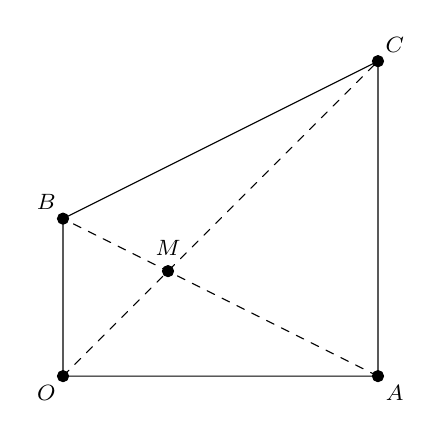
\begin{tikzpicture}[scale=1, line join=round, line cap=round, >=stealth, font=\footnotesize]
					\coordinate (O) at (0,0);
					\coordinate (A) at (4,0);
					\coordinate (B) at (0,2);
					\coordinate (C) at (4,4);
					\coordinate (M) at (intersection of O--C and A--B);
					
					\draw (O) -- (A) -- (C) -- (B) -- cycle;
					\draw[dashed] (O) -- (C) (A) -- (B);
					
					\foreach \p/\g in {O/-135, A/-45, B/135, C/45, M/90} {
						\filldraw (\p) circle (2pt) node[shift={(\g:3mm)}]{$\p$};
					}
				\end{tikzpicture}
			}
			\noindent
			Điều này chứng tỏ tia $OC$ nằm giữa hai tia $OA$ và $OB$, nên tứ giác $OACB$ là tứ giác lồi nhận $OC$ và $AB$ làm hai đường chéo.\\
			Tổng khoảng cách $S = MA + MB + MC + MO$ đạt giá trị nhỏ nhất khi $M$ là giao điểm của hai đường chéo $AB$ và $OC$.\\
			Khi đó $S_{\min} = AB + OC$.\\
			Ta có $AB = \sqrt{(2-0)^2 + (0-1)^2 + (1-1)^2}= \sqrt{5}$ và $OC = \sqrt{2^2 + 2^2 + 3^2} = \sqrt{17}$.\\
			Vậy giá trị nhỏ nhất là $\sqrt{5} + \sqrt{17} \approx 6{,}4$.
		\end{itemchoice}
	}
\end{ex}
%%%=============================%%%

%%%=============EX_14=============%%%
\begin{ex}%[2D1V3-1]%[TDMT08]%[Vũ Hồng Toàn]
	Cho hàm số $f(x) = x + \cos x - \sqrt{3} \sin x$.
	\choiceTF
	{$f'(x)=1+\sin x-\sqrt{3}\cos x$}
	{\True $f'(x)=1-2\sin \left( x+\dfrac{\pi}{3} \right)$}
	{\True $f'\left(\dfrac{\pi}{2}\right)=0$}
	{\True $\min\limits_{[0;\pi]} f(x)=\dfrac{\pi-2\sqrt{3}}{2}$}
	\loigiai{
		\begin{itemchoice}
			\itemch Ta có $f(x) = x + \cos x - \sqrt{3} \sin x\Rightarrow f'(x) = 1 - \sin x - \sqrt{3} \cos x$.
			\itemch Ta có
			\allowdisplaybreaks
			\begin{align*}
				f'(x) &= 1 - \sin x - \sqrt{3} \cos x\\
				&= 1 - \left(\sin x + \sqrt{3} \cos x\right)\\
				&= 1-2\left(\sin x \cdot \dfrac{1}{2} + \cos x \cdot \dfrac{\sqrt{3}}{2}\right)\\
				&= 1-2 \left( \sin x \cos \dfrac{\pi}{3} + \cos x \sin \dfrac{\pi}{3} \right)\\
				&= 1-2\sin \left( x+\dfrac{\pi}{3} \right).
			\end{align*}
			\itemch Vì $f'(x) = 1 - \sin x - \sqrt{3} \cos x$.\\
			Nên $f'\left(\dfrac{\pi}{2}\right) = 1 - \sin\left(\dfrac{\pi}{2}\right) - \sqrt{3} \cos\left(\dfrac{\pi}{2}\right)=1 - 1 - \sqrt{3} \cdot 0 = 0$.
			\itemch Ta có $f'(x) = 1 - 2\sin\left(x+\dfrac{\pi}{3}\right)$.
			\allowdisplaybreaks
			\begin{align*}
				& f'(x) = 0\\
				\Leftrightarrow & 1 - 2\sin\left(x+\dfrac{\pi}{3}\right) = 0\\
				\Leftrightarrow & \sin\left(x+\dfrac{\pi}{3}\right) = \dfrac{1}{2}\\
				\Leftrightarrow & \hoac{& x+\dfrac{\pi}{3}=\dfrac{\pi}{6}+k2\pi\\ & x+\dfrac{\pi}{3}=\pi-\dfrac{\pi}{6}+k2\pi} \quad (k\in\mathbb{Z})\\
				\Leftrightarrow & \hoac{& x=-\dfrac{\pi}{6}+k2\pi\\ & x=\dfrac{\pi}{2}+k2\pi} \quad (k\in\mathbb{Z}).
			\end{align*}
			\begin{itemize}
				\item Xét $x=-\dfrac{\pi}{6}+k2\pi$.\\
				Vì $x \in [0;\pi]$ nên $0\le -\dfrac{\pi}{6}+k2\pi\le \pi\Leftrightarrow 0\le -\dfrac{1}{6}+2k\le 1\Leftrightarrow \dfrac{1}{12}\le k\le \dfrac{7}{12}$.\\
				Do $k\in\mathbb{Z}$ nên không tồn tại giá trị $k$ thỏa mãn.
				\item Xét $x=\dfrac{\pi}{2}+k2\pi$.\\
				Vì $x \in [0;\pi]$ nên $0\le \dfrac{\pi}{2}+k2\pi\le \pi\Leftrightarrow 0\le \dfrac{1}{2}+2k\le 1\Leftrightarrow -\dfrac{1}{4}\le k\le \dfrac{1}{4}$.\\
				Do $k\in\mathbb{Z}\Rightarrow k=0\Rightarrow x=\dfrac{\pi}{2}$.
			\end{itemize}
			Khi đó $f(0)= 1$; $f(\pi) = \pi - 1 \approx 2{,}14$; $f\left(\dfrac{\pi}{2}\right) = \dfrac{\pi-2\sqrt{3}}{2} \approx -0{,}16$.\\
			So sánh các giá trị ta thấy $f\left(\dfrac{\pi}{2}\right)$ nhỏ nhất.\\
			Vậy $\min\limits_{[0;\pi]} f(x)=\dfrac{\pi-2\sqrt{3}}{2}$.
		\end{itemchoice}
	}
\end{ex}
%%%=============================%%%

%%%=============EX_15=============%%%
\begin{ex}%[2H2H2-6]%[TDMTD09]%[Dương Công Tạo]
	Trong không gian $Oxyz$, một vật có trọng lượng $P=360\mathrm{\,N}$ được treo bằng ba sợi dây cáp không giãn, các dây cáp có một đầu được gắn tương ứng tại các điểm $A(1;0;0)$, $B(3;0;0)$, $C(2;2;0)$ và đầu còn lại gắn chung vào một điểm $D(2;1;-2)$. Biết rằng trọng lực $\overrightarrow{P}=(0;0;-6)$ sẽ kéo vào ba sợi dây tạo ra ba lực căng trên các sợi dây là $\overrightarrow{T}_1$, $\overrightarrow{T}_2$, $\overrightarrow{T}_3$ lần lượt hướng dọc theo các vectơ $\overrightarrow{AD}$, $\overrightarrow{BD}$, $\overrightarrow{CD}$. Theo tính chất Vật Lý thì ta có $\overrightarrow{T}_1+\overrightarrow{T}_2+\overrightarrow{T}_3=\overrightarrow{P}$.
	\begin{center}
		\begin{tikzpicture}[>=stealth, font=\footnotesize, line join=round, line cap=round]			
			\coordinate (D) at (4, 1.5); 			
			\coordinate (A) at (2, 5);  			
			\coordinate (B) at (4.5, 5.8);			
			\coordinate (C) at (7, 5.2); 			
			
			\filldraw[fill=blue!15, draw=black!40, opacity=0.7] (-0.5, 4.2) -- (2.5, 6.8) -- (10.5, 6.8) -- (7.5, 4.2) -- cycle;			
			
			\foreach \p in {A, B, C} {				
				\draw[black!60, fill=black!20] (\p) ellipse (0.15 and 0.07);
			}			
			
			\draw[red, thick] (A) -- (D);			
			\draw[red, thick] (B) -- (D);			
			\draw[red, thick] (C) -- (D);			
			
			\draw[blue, ultra thick, ->] (A) -- ($(A)!0.3!(D)$);			
			\node[left, blue] at ($(A)!0.2!(D)$) {$\overrightarrow{T}_1$};			
			\draw[blue, ultra thick, ->] (B) -- ($(B)!0.2!(D)$);			
			\node[right, blue] at ($(B)!0.1!(D)$) {$\overrightarrow{T}_2$};			
			\draw[blue, ultra thick, ->] (C) -- ($(C)!0.25!(D)$);			
			\node[right, blue] at ($(C)!0.15!(D)$) {$\overrightarrow{T}_3$};			
			
			\node[above left] at (A) {$A$};			
			\node[above] at (B) {$B$};			
			\node[above right] at (C) {$C$};			
			
			\filldraw (D) circle (1.8pt) node[right, xshift=2pt] {$D$};			
			
			\begin{scope}[shift={(3.5,-0.2)}]				
				\draw[thick, fill=white] (0,0) rectangle (1,0.8); 				
				\draw[thick, fill=gray!10] (1,0) -- (1.3,0.3) -- (1.3,1.1) -- (1,0.8) -- cycle;			
				\draw[thick, fill=gray!5] (0,0.8) -- (0.3,1.1) -- (1.3,1.1) -- (1,0.8) -- cycle; 				
				\node at (0.5,0.4) {$360\mathrm{\,N}$};				
				\draw[red, thick] (D)--(.5,.95);
				\filldraw (0.5,0.95) circle (2pt);			
			\end{scope}			
			
			\draw[blue, ultra thick, ->] (4, -0.2) -- (4, -1.2) node[right] {$\overrightarrow{P}$};			
		\end{tikzpicture}
	\end{center}
	\choiceTF[t]
	{\True Một đơn vị dài trong hệ trục tọa độ $Oxyz$ tương ứng với độ lớn của lực là $60\mathrm{\,N}$}
	{\True Ba điểm $A$, $B$, $C$ cùng thuộc mặt phẳng tọa độ $(Oxy)$}
	{\True Tọa độ vectơ lực căng $\overrightarrow{T}_1=(k; k;-2k)$, $k \in \mathbb{R}$, $k > 0$}
	{Độ lớn của lực $\overrightarrow{T}_2$ trong thực tế bằng $131\mathrm{\,N}$ (tính theo đơn vị Newton và \textit{làm tròn kết quả đến hàng đơn vị})}
	\loigiai{
		\begin{itemchoice}
			\itemch Ta có $\overrightarrow{P}=(0;0;-6)$ suy ra $\left|\overrightarrow{P}\right|=6$ (đvđd).\\
			Mà vật có trọng lượng $P=360\mathrm{\,N}$ nên một đơn vị dài trong hệ trục tọa độ $Oxyz$ tương ứng với độ lớn của lực là $360:6=60\mathrm{\,N}$.
			\itemch Ta có $z_A=z_B=z_C=0$ nên ba điểm $A$, $B$, $C$ cùng thuộc mặt phẳng tọa độ $(Oxy)$.
			\itemch Vì $\overrightarrow{T}_1$ có giá thuộc đường thẳng $AD$ nên $\overrightarrow{T}_1=k\cdot\overrightarrow{AD}=(k; k;-2k)$, $k \in \mathbb{R}$, $k > 0$.
			\itemch Ta có $\overrightarrow{AD}=(1;1;-2)$, $\overrightarrow{BD}=(-1;1;-2)$ và $\overrightarrow{CD}=(0;-1;-2)$.\\
			Theo giả thiết, ta có
			\allowdisplaybreaks
			\begin{align*}
				& \overrightarrow{T}_1+\overrightarrow{T}_2+\overrightarrow{T}_3=\overrightarrow{P}\\
				\Leftrightarrow & a\cdot\overrightarrow{AD}+b\cdot\overrightarrow{BD}+c\cdot\overrightarrow{CD}=\overrightarrow{P}\\
				\Leftrightarrow & \heva{&a-b=0\\&a+b-c=0\\&-2a-2b-2c=-6} \Leftrightarrow\heva{&a=\dfrac{3}{4}\\&b=\dfrac{3}{4}\\&c=\dfrac{3}{2}.}
			\end{align*}
			Khi đó $\left|\overrightarrow{T}_2\right|=\left|b\right|\cdot\left|\overrightarrow{BD}\right|=\dfrac{3}{4}\cdot\sqrt{6}=\dfrac{3\sqrt{6}}{4}$.\\
			Vậy, độ lớn của lực $\overrightarrow{T}_2$ trong thực tế là $\dfrac{3\sqrt{6}}{4}\cdot 60\approx 110\mathrm{\,N}$.
		\end{itemchoice}
	}
\end{ex}
%%%=============================%%%

%%%=============EX_16=============%%%
\begin{ex}%[2D1H3-6]%[TDMT09]%[Văn Minh Thoại]
	Một phương tiện giao thông trên bộ có vận tốc tối đa là $150\mathrm{\,km/h}$. Chi phí về nhiên liệu của phương tiện gồm có hai phần là phần thứ nhất chỉ phụ thuộc vào thời gian nổ máy và có chi phí bằng $120$ nghìn đồng/giờ; phần thứ hai có chi phí trên $1$ kilômét đường tỉ lệ với bậc hai của vận tốc của phương tiện đi trên quãng đường đó và khi vận tốc bằng $20\mathrm{\,km/h}$ thì chi phí phần thứ hai này là $80$ nghìn đồng/giờ.
	\choiceTF[t]
	{\True Trong hai giờ nổ máy chi phí phần thứ nhất bằng $240$ nghìn đồng}
	{\True Chi phí phần thứ hai là $0{,}01v^2$ (nghìn đồng/km), với $v$ tính theo $\mathrm{km/h}$}
	{\True Tổng chi phí khi phương tiện đi được $1\mathrm{\,km}$ với vận tốc $v$ là $\dfrac{120}{v}+0{,}01v^2$ (nghìn đồng)}
	{\True Tổng chi phí nhỏ nhất của phương tiện để đi được $10\mathrm{\,km}$ là $99$ nghìn đồng \textit{(tính theo đơn vị nghìn đồng và làm tròn kết quả đến hàng đơn vị)}}
	\loigiai{
		\begin{itemchoice}
			\itemch Chi phí phần thứ nhất trong $2$ giờ là $120 \cdot 2 = 240$ (nghìn đồng).
			\itemch Gọi chi phí phần thứ hai trên $1\mathrm{\,km}$ là $f(v) = kv^2$ (nghìn đồng/km).\\
			Theo bài ra, khi $v=20\mathrm{\,km/h}$, chi phí phần này là $80$ nghìn đồng/giờ.\\
			Trong $1$ giờ phương tiện đi được $20\mathrm{\,km}$, nên chi phí trên $1\mathrm{\,km}$ là $\dfrac{80}{20} = 4$ (nghìn đồng/km).\\
			Ta có $k \cdot 20^2 = 4 \Rightarrow k = \dfrac{4}{400} = 0{,}01$.\\
			Vậy chi phí phần thứ hai là $0{,}01v^2$ (nghìn đồng/km).
			\itemch Thời gian để đi được $1\mathrm{\,km}$ với vận tốc $v$ là $t = \dfrac{1}{v}$ (giờ).\\
			Tổng chi phí cho $1\mathrm{\,km}$ là
			\[T(v) = 120 \cdot \dfrac{1}{v} + 0{,}01v^2 = \dfrac{120}{v} + 0{,}01v^2.\]
			\itemch Tổng chi phí cho $10\mathrm{\,km}$ là $G(v) = 10 \cdot \left( \dfrac{120}{v} + 0{,}01v^2 \right) = \dfrac{1\,200}{v} + 0{,}1v^2$.\\
			Xét $G'(v) = -\dfrac{1\,200}{v^2} + 0{,}2v$.\\
			Cho $G'(v) = 0 \Leftrightarrow 0{,}2v^3 = 1\,200 \Leftrightarrow v^3 = 6\,000 \Rightarrow v = \sqrt[3]{6\,000}\mathrm{\,km/h}$.\\
			Khi đó giá trị nhỏ nhất là $G\left(\sqrt[3]{6\,000}\right) = \dfrac{1\,200}{\sqrt[3]{6\,000}} + 0{,}1 \cdot \left(\sqrt[3]{6\,000}\right)^2\approx 99$.
		\end{itemchoice}
	}
\end{ex}
%%%=============================%%%
\Closesolutionfile{ans}

\caukq 
\Opensolutionfile{ans}[ans/ansTN-DienKhuyet]
%%=============EX_17=============%%%
\begin{ex}%[TDMT09]%[Lương Pho]%[1H8H5-4]
	Cho hình chóp đều $S.ABCDEF$ có độ dài các cạnh $SA = 8$, $AB = 6$. Hãy tính khoảng cách giữa hai đường thẳng $SA$ và $CD$ (\textit{làm tròn kết quả đến hàng phần mười}).
	\par\shortans[0]{7{,}4}
	\loigiai{
		\immini{
			Gọi $O$ là tâm lục giác đều $ABCDEF$; $I$, $H$ lần lượt là hình chiếu $O$ lên $AF$ và $SI$.\\
			Ta có $\heva{&AF \perp SO \\ & AF \perp OI}\Rightarrow AF \perp (SOI)\Rightarrow AF \perp OH$.\\
			Lại có $\heva{&OH \perp SI \\& OH \perp AF} \Rightarrow OH \perp (SAF)$.\\
			Do $CD \parallel AF \Rightarrow CD \parallel (SAF)$.\\
			Suy ra $\mathrm{d}(SA, CD)=\mathrm{d}\big(D,(SAF)\big)=2\mathrm{d}\big(O,(SAF)\big)=2OH$.\\
			Tam giác $AOF$ đều cạnh $AF=AB=6\Rightarrow OI=3\sqrt{3}$.\\
			Trong tam giác $SAO$, ta có \[SO=\sqrt{SA^2-OA^2}=\sqrt{8^2-6^2}=2\sqrt{7}.\]
			Trong tam giác $SOI$, ta có
			\[OH=\dfrac{SO\cdot OI}{\sqrt{SO^2+OI^2}}=\dfrac{6\sqrt{21}}{\sqrt{55}}.\]
			Vậy $\mathrm{d}(SA, CD)=2OH=\dfrac{12\sqrt{21}}{\sqrt{55}}\approx 7{,}4$.
		}{
			\begin{tikzpicture}[declare function={k=1.4; a=k*4; h=0.8*a; xien=-55;}, font=\footnotesize, line join=round, line cap=round, >=stealth]
				\path
				(0,0) coordinate (A)
				(a,0) coordinate (D)
				(xien:0.45*a) coordinate (B)
				($(B)+(0.5*a,0)$) coordinate (C)
				($(A)!.5!(D)$) coordinate (O)
				($2*(O)-(C)$) coordinate (F)
				($2*(O)-(B)$) coordinate (E)			
				($(O)+(90:1.1*a)$) coordinate (S)
				($(A)!.5!(B)$) coordinate (I)
				($(S)!.7!(I)$) coordinate (H);
				
				\draw (S)--(A) (S)--(B) (S)--(C) (S)--(D) (S)--(I) (A)--(B)--(C)--(D);
				\draw[dashed] (A)--(O) (S)--(O)--(H) (O)--(I) (O)--(E) (A)--(F)--(E)--(D) (S)--(E) (S)--(F) (O)--(B);
				
				\foreach \x/\g/\nhan in {A/200/F, B/-90/A, C/-30/B, D/0/C, E/20/D, F/160/E, O/-30/O, S/160/S, I/180/I, H/180/H} {
					\filldraw (\x) circle (1pt) node[shift={(\g:3mm)}]{\nhan};
				}
				
				\path pic[draw,angle radius=2mm]{right angle=O--I--B};
				\path pic[draw,angle radius=2mm]{right angle=S--O--I};
				\path pic[draw,angle radius=2mm]{right angle=O--H--I};
			\end{tikzpicture}
		}
	}
\end{ex}
%%%=============================%%%

%%%=============EX_18=============%%%
\begin{ex}%[1D7V1-5] %[TDMT09]%[Hà Văn Hảo]
	Cho một quần thể vi khuẩn được nghiên cứu trong phòng thí nghiệm tăng trưởng theo quy luật $R(t) = a\sqrt{t^2 + 20t + 1\,600} - b\dfrac{t^2 + 3t + 100}{t + 1}$ (vi khuẩn), thời gian $t$ tính theo giờ. Biết ban đầu có $2\,000$ vi khuẩn và khi thời gian đủ lớn ($t > 10\,000$ giờ) nó tăng trưởng với tốc độ $200$ vi khuẩn/giờ. Hãy xác định số lượng vi khuẩn có được sau $24$ giờ tính theo đơn vị nghìn con (\textit{làm tròn kết quả đến hàng phần mười}).
	\par
	\shortans[0]{12{,}5}
	\loigiai{
		Tại thời điểm $t=0$, số lượng vi khuẩn là $2\,000$, ta có
		\[R(0) = a\sqrt{1\,600} - b\dfrac{100}{1} = 2\,000 \Leftrightarrow 2a - 5b = 100. \quad (1)\]
		Khi $t$ đủ lớn, tốc độ tăng trưởng tức thời $R'(t)$ với vận tốc $200$ vi khuẩn/giờ. Ta có
		\allowdisplaybreaks
		\begin{align*}
			\lim\limits_{t \to +\infty} \dfrac{R(t)}{t} = 200 &\Leftrightarrow \lim\limits_{t \to +\infty} \left( a\sqrt{1 + \dfrac{20}{t} + \dfrac{1\,600}{t^2}} - b\dfrac{1 + \dfrac{3}{t} + \dfrac{100}{t^2}}{1 + \dfrac{1}{t}} \right) = 200\\
			&\Leftrightarrow a - b = 200. \quad (2)
		\end{align*}
		Từ $(1)$ và $(2)$ ta có hệ phương trình
		\[\heva{&2a - 5b = 100 \\ &a - b = 200 } \Leftrightarrow \heva{&a = 300 \\ &b = 100.}\]
		Số lượng vi khuẩn sau $24$ giờ là
		\allowdisplaybreaks
		\begin{align*}
			R(24) &= 300\sqrt{24^2 + 20 \cdot 24 + 1\,600} - 100\cdot \dfrac{24^2 + 3 \cdot 24 + 100}{24 + 1}\\
			&= 300\sqrt{2\,656} - 100\cdot \dfrac{748}{25}\\
			&\approx 12\,468{,}8 \text{ (vi khuẩn)}.
		\end{align*}
		Vậy số lượng vi khuẩn có được sau $24$ giờ là $12{,}5$ nghìn con.
	}
\end{ex}
%%%=============================%%%

%%%=============EX_19=============%%%
\begin{ex}%[1C2V3-1]%[TDMT09]%[Võ Hiệp]
	\immini[thm]{Một trò chơi điện tử quy định như sau: Có $8$ trụ $A$, $B$, $C$, $D$, $E$, $F$, $G$, $H$ với số lượng các thử thách trên đường đi giữa các cặp trụ được mô tả trong hình bên. Người chơi xuất phát từ một trụ nào đó, đi qua tất cả các trụ còn lại, mỗi lần đi qua một trụ thì trụ đó sẽ bị phá hủy và không thể quay trở lại trụ đó được nữa, nhưng người chơi vẫn phải quay trở về trụ ban đầu. Tổng số thử thách của đường đi thoả mãn điều kiện trên nhận giá trị nhỏ nhất là bao nhiêu?
	}{
		\begin{tikzpicture}[scale=1, >=stealth, font=\footnotesize, line join=round, line cap=round]
			\def\h{2.5}
			\path
			(0,0) coordinate (A) 
			(3,0) coordinate (D)
			(-120:2) coordinate (B)
			($(B)+(D)-(A)$) coordinate (C)
			($(A)+(0,\h)$) coordinate (E)
			($(B)+(0,\h)$) coordinate (F)
			($(C)+(0,\h)$) coordinate (G)
			($(D)+(0,\h)$) coordinate (H);
			
			\draw (E)--node[midway,left]{$13$}(F)--node[midway,below]{$6$}(G)--node[midway,right]{$6$}(H)--node[midway,above]{$14$}cycle 
			(B)--node[midway,below]{$7$}(C)--node[midway,right]{$5$}(D)
			(B)--node[midway,left]{$6$}(F) (C)--node[midway,right]{$4$}(G) (D)--node[midway,right]{$9$}(H);
			
			\draw[dashed] (B)--node[midway,right]{$6$}(A)--node[midway,below]{$8$}(D) (A)--node[midway,left]{$7$}(E);
			
			\foreach \d/\g in{A/150, B/-150, C/-60, D/-30, E/135, F/180, G/135, H/30} {
				\filldraw (\d) circle (1pt) node[shift={(\g:3mm)}]{$\d$};
			}
		\end{tikzpicture}
	}
	\par
	\shortans[0]{57}
	\loigiai{
		Dựa vào hình vẽ, ta có danh sách các cạnh và trọng số tương ứng là\\
		Mặt đáy $AB=6$, $BC=7$, $CD=5$, $DA=8$.\\
		Mặt trên $EF=13$, $FG=6$, $GH=6$, $HE=14$.\\
		Các cạnh đứng $AE=7$, $BF=6$, $CG=4$, $DH=9$.\\
		Do mỗi đỉnh có bậc $3$ (nối với $3$ cạnh), trong chu trình, mỗi đỉnh sẽ sử dụng đúng $2$ cạnh nối với nó.
		Để tổng số thử thách là nhỏ nhất, ta nên ưu tiên chọn các cạnh có giá trị thấp và tránh các cạnh có giá trị lớn.
		Một số lộ trình đi qua tất cả các đỉnh là
		\begin{itemize}
			\item Lộ trình 1: $A \to B \to F \to E \to H \to G \to C \to D \to A$.\\
			Tổng: $AB + BF + FE + EH + HG + GC + CD + DA=6 + 6 + 13 + 14 + 6 + 4 + 5 + 8 = 62$.
			\item Lộ trình 2: $A \to E \to F \to G \to H \to D \to C \to B \to A$.\\
			Tổng: $AE + EF + FG + GH + HD + DC + CB + BA=7 + 13 + 6 + 6 + 9 + 5 + 7 + 6 = 59$.
			\item Lộ trình 3: $A \to B \to F \to G \to C \to D \to H \to E \to A$.\\
			Tổng:= $AB + BF + FG + GC + CD + DH + HE + EA=6 + 6 + 6 + 4 + 5 + 9 + 14 + 7 = 57$.
			\item Lộ trình 4: $A \to D \to C \to G \to F \to B \to A \dots$ (không thể nối thêm $E$, $H$ mà không tăng trọng số lớn).
		\end{itemize}
		Vậy tổng số thử thách nhỏ nhất của đường đi thỏa mãn điều kiện đề bài là $57$.
	}
\end{ex}
%%%=============================%%%

%%%=============EX_20=============%%%
\begin{ex}%[2D1V3-6]%[TDMT09]%[Nguyễn Đức Tuấn Anh]
	Giả sử giá của một cổ phiếu nào đó (tính bằng USD) trong một ngày nhất định (có $8$ giờ giao dịch tính từ $8$ giờ sáng đến $16$ giờ chiều) được mô tả bởi hàm số
	\[f(x) = \heva{&48{,}8 & \text{khi } 0 \le x < 2 \\ &0{,}3x^4 - 5{,}2x^3 + 30x^2 - 67{,}2x + 100 & \text{khi } 2 \le x \le 8}\text{ (USD).}\]
	Trong đó $x$ là thời gian (giờ) tính từ khi sàn giao dịch mở cửa, ở thời điểm $8$ giờ sáng ứng với $x=0$, ở thời điểm $16$ giờ chiều ứng với $x=8$. Nếu một người dự tính sẽ mua $400$ cổ phiếu và bán chúng ngay trong ngày này thì người đó có lợi nhuận tối đa là bao nhiêu USD (\textit{làm tròn kết quả đến hàng đơn vị})?
	\par\shortans[0]{5000}
	\loigiai{
		Với $x \in [2;8]$, ta có $f'(x) = 1{,}2x^3 - 15{,}6x^2 + 60x - 67{,}2$.\\
		Khi đó $f'(x) = 0 \Leftrightarrow x \in \{2; 4; 7\}$.\\
		Bảng biến thiên
		\begin{center}
			\begin{tikzpicture}
				\tkzTabInit[lgt=1.25,espcl=2.5,deltacl=0.5]
				{$x$/1, $f'(x)$/1, $f(x)$/3}
				{$0$,$2$,$4$,$7$,$8$}
				\tkzTabLine{,,z,+,0,-,z,+,}
				\draw 
				($(N12)!0.5!(N13)$) node (A){$48{,}8$}
				($(N22)!0.5!(N23)$) node (B){$48{,}8$}
				(N32)node[below](C){$55{,}2$}
				(N43)node[above](D){$36{,}3$}
				($(N52)!0.5!(N53)$) node (E){$48{,}8$}
				;
				\foreach \x/\y in {A/B,B/C,C/D,D/E}{\draw[-stealth] (\x)--(\y);}
			\end{tikzpicture}
		\end{center}
		Quan sát bảng biến thiên, ta có hai phương án giao dịch khả thi
		\begin{itemize}
			\item \textit{Phương án 1}: Mua giá $48{,}8$ (lúc $x<2$) và bán giá cực đại $55{,}2$ (lúc $x=4$).\\
			Lợi nhuận $400 \cdot (55{,}2 - 48{,}8) = 2\,560$ (USD).
			\item \textit{Phương án 2}: Mua giá cực tiểu $36{,}3$ (lúc $x=7$) và bán giá cuối ngày $48{,}8$ (lúc $x=8$).\\
			Lợi nhuận $400 \cdot (48{,}8 - 36{,}3) = 5\,000$ (USD).
		\end{itemize}
		So sánh hai phương án, ta thấy lợi nhuận tối đa là $5\,000$ USD.
	}
\end{ex}
%%%=============================%%%

%%%=============EX_21=============%%%
\begin{ex}%[1H8V7-9]%[TDMT09]%[Lê Hồ Quang Minh]
	\immini[thm]{Cho một phòng khách dạng hình hộp chữ nhật $ABCD.A'B'C'D'$ có độ dài các cạnh $AD = 6\mathrm{\,m}$, $AA' = 4\mathrm{\,m}$, $AB = 5\mathrm{\,m}$. Người ta muốn đi một đường dây từ điểm $B$ đến điểm $D'$ sao cho từ $B$ đường dây đến chạm vào mặt bức tường $(CDD'C')$ tại điểm $M$ và từ $D'$ đường dây đến chạm vào cạnh trần $A'B'$ tại điểm $N$. Tính độ dài ngắn nhất của đường dây theo đơn vị mét \textit{(làm tròn kết quả đến hàng phần mười)}.}{
		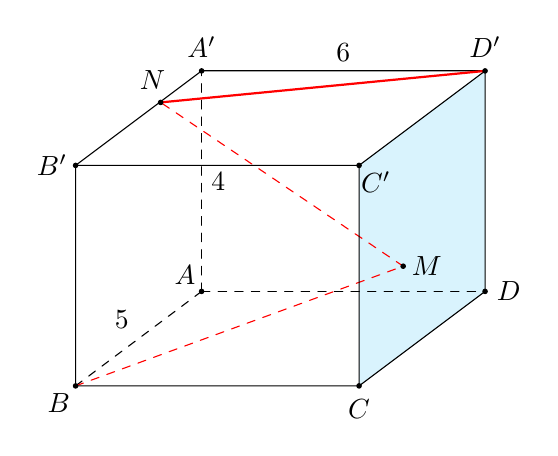
\begin{tikzpicture}[scale=0.8, line join=round, line cap=round, >=stealth]
			\coordinate (A) at (2,1.5);
			\coordinate (B) at (0,0);
			\coordinate (C) at (4.5,0);
			\coordinate (D) at (6.5,1.5);
			
			\coordinate (A') at (2,5);
			\coordinate (B') at (0,3.5);
			\coordinate (C') at (4.5,3.5);
			\coordinate (D') at (6.5,5);
			
			\coordinate (N) at (1.35, 4.5);
			\coordinate (M) at (5.2, 1.9);
			
			\fill[cyan!15] (C)--(D)--(D')--(C')--cycle;
			
			\draw[dashed] (A)--(D) (A)--(A');
			\draw[dashed] (A)--(B) node[midway, above left] {$5$}; 
			\draw[dashed] (A)--(A') node[midway, right] {$4$};    
			\draw[dashed, red] (B)--(M)--(N);
			
			\draw (B)--(C)--(D) (C)--(C') (D)--(D') (B)--(B');
			\draw (A')--(B')--(C')--(D')--cycle;
			\draw (A')--(D') node[midway, above] {$6$}; 
			
			\draw[red, thick] (N)--(D');
			
			\foreach \x/\g in {A/135, B/-135, C/-90, D/0, A'/90, B'/180, C'/-45, D'/90, M/0, N/110} {
				\filldraw (\x) circle (1pt) node[shift={(\g:3mm)}]{$\x$};
			}
		\end{tikzpicture}
	}
	\par\shortans[0]{19{,}3}
	\loigiai{
		\begin{center}
			\begin{tikzpicture}[scale=0.75, line join=round, line cap=round, >=stealth]
				\coordinate (A) at (2,1.5);
				\coordinate (B) at (0,0);
				\coordinate (C) at (4.5,0);
				\coordinate (D) at (6.5,1.5);
				
				\coordinate (A') at (2,5.5);
				\coordinate (B') at (0,4);
				\coordinate (C') at (4.5,4);
				\coordinate (D') at (6.5,5.5);
				
				\coordinate (N) at (1.35, 5);
				\coordinate (M) at (5.2, 1.9);
				\coordinate (I) at ($(D)!0.5!(D')$); 
				
				\coordinate (B_1) at ($2*(C)-(B)$);
				\coordinate (A_1) at ($2*(D)-(A)$);
				\coordinate (D_1) at ($3/2*(A')-1/2*(A_1)$);
				\coordinate (C_1) at ($3/2*(B')-1/2*(B_1)$);
				
				\fill[cyan!15] (C)--(D)--(D')--(C')--cycle;
				
				\draw[dashed] (B)--(A)--(D) (A)--(A');
				\draw[dashed] (A)--(B) node[midway, above left] {$5$};
				\draw[dashed] (A)--(A') node[midway, right] {$4$};
				\draw[dashed] (D)--(A_1) (A')--(I);
				\draw[dashed, red] (B)--(M)--(N) (M)--(B_1)--(D_1);
				
				\draw (B)--(C)--(D) (C)--(C') (D)--(D') (B)--(B');
				\draw (A')--(B')--(C')--(D')--cycle;
				\draw (A')--(D') node[midway, above] {$6$};
				\draw (C)--(B_1)--(A_1)--(I);
				\draw (A')--(D_1) (B_1)--(C_1)--(D_1);
				
				\draw[red, thick] (N)--(D');
				
				\foreach \x/\g in {A/135, B/180, C/-90, D/45, A'/135, B'/180, C'/-45, D'/45, M/-90, N/-90, I/40, A_1/0, B_1/-90, C_1/180, D_1/90} {
					\filldraw (\x) circle (1pt) node[shift={(\g:3.5mm)}]{$\x$};
				}
			\end{tikzpicture}
		\end{center}
		Tổng độ dài của đường dây là $T=BM+MN+ND'$.\\
		Gọi $B_1$ đối xứng với $B$ qua mặt phẳng $(CC'D'D)$. Suy ra $BM=B_1M$.\\
		Gọi $D_1$ là ảnh của $D'$ quay quanh đường thẳng $A'B'$.\\
		Trong các ảnh trên ta chọn $1$ ảnh thuộc mặt phẳng $(A'B'B_1A_1)$, với $A_1$ là điểm đối xứng của $A$ qua $D$.\\
		Suy ra $ND'=ND_1$.\\
		Khi đó $T=MB_1+MN+ND_1 \geq B_1D_1$.\\
		$A'A_1=\sqrt{AA_1^2+A'A^2}=4\sqrt{10}$.\\
		Suy ra $A_1D_1=4\sqrt{10}+6$.\\
		Tam giác $A_1B_1D_1$ vuông tại $A_1$ nên $B_1D_1=\sqrt{A_1D_1^2+A_1B_1^2} \approx 19{,}3$.
	}
\end{ex}
%%%=============================%%%

%%%=============EX_22=============%%%
\begin{ex}%[0D8C1-3]%[TDMT09]%[Nguyễn Thành Hậu]
	\immini[thm]{Một bạn học sinh tên Hùng dùng $4$ màu sắc khác nhau để tô $8$ hình tròn $A$, $B$, $C$, $D$, $E$, $F$, $G$, $H$ như hình vẽ bên dưới sao cho mỗi hình tròn được tô một màu. Hãy đếm cách tô màu khác nhau của bạn Hùng thỏa mãn hai hình tròn nối với nhau được tô bởi hai màu khác nhau.}{
		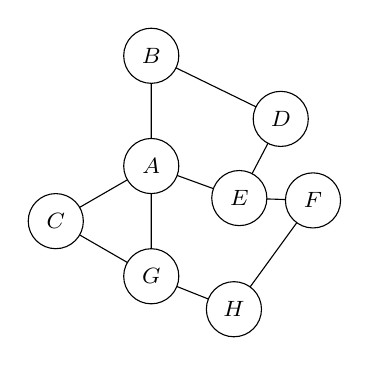
\begin{tikzpicture}[declare function={r=0.5;}, line cap=round, line join=round, >=stealth, font=\footnotesize, scale=0.7]
			\path (0,0) coordinate (A) 
			(90:2) coordinate (B)
			(20:2.5) coordinate (D)
			(-20:1.7) coordinate (E)
			(-90:2) coordinate (G)
			(-150:2) coordinate (C)
			(-12:3) coordinate (F)
			(-60:3) coordinate (H);
			
			\draw (A) -- (B) -- (D) -- (E) -- cycle;
			\draw (A) -- (G) -- (C) -- cycle;	
			\draw (E) -- (F) -- (H) -- (G);
			
			\foreach \u in {A,B,C,D,E,F,H,G} {
				\filldraw[fill=white, draw=black] (\u) circle (r);
				\node at (\u) {$\u$};
			}
	\end{tikzpicture}}
	\par
	\shortans[0]{3360}
	\loigiai{Trước tiên ta tính số cách tô màu các hình tròn $A$, $E$, $F$, $H$, $G$ nối vòng tròn với nhau theo thứ tự đó và thỏa mãn yêu cầu.
		\begin{itemize}
			\item \textbf{Trường hợp 1.} $A$ và $H$ khác màu.\\
			Tô màu cho $A$ có $4$ cách, tô màu cho $H$ có $3$ cách (khác màu với $A$), tô màu cho $G$ có $2$ cách (khác màu với $H$ và $A$).\\
			Nếu $E$ cùng màu với $H$ thì $E$ có $1$ cách tô, $F$ có $3$ cách tô. Do đó có $4\cdot 3\cdot 2\cdot 1\cdot 3=72$ cách tô.\\
			Nếu $E$ khác màu với $H$, $E$ có $2$ cách tô (khác màu với $A$ và $H$), $F$ có $2$ cách tô. Do đó có $4\cdot 3\cdot 2\cdot 2\cdot 2=96$ cách tô.\\
			Trường hợp này có $72+96=168$ cách tô.
			\item \textbf{Trường hợp 2.} $A$ và $H$ cùng màu.\\
			Tô màu cho hai $A$ và $H$ có $4$ cách.\\
			Chọn ra hai màu khác trong $3$ màu còn lại và tô cho $E$ và $F$ có $\mathrm{A}_{3}^{2}=6$ cách tô. Tô màu cho $G$ có $3$ cách tô.\\
			Trường hợp này có $4\cdot 6 \cdot 3=72$ cách tô.
		\end{itemize}
		Như thế, có $168+72=240$ cách tô màu các hình tròn $A$, $E$, $F$, $H$, $G$ thỏa mãn yêu cầu.\\
		Với mỗi cách tô như trên, ta sẽ tính số cách tô các hình tròn còn lại (hình tròn $C$, $B$, $D$) thỏa mãn yêu cầu.\\
		Tô màu cho $C$ có $2$ cách (khác màu với $A$ và $G$).\\
		Nếu $B$ cùng màu với $E$ thì $B$ có $1$ cách tô, $D$ có $3$ cách tô. Như vậy trường hợp này có $1\cdot 3=3$ cách tô màu cho $B$ và $D$.\\
		Nếu $B$ khác màu với $E$ thì $B$ có $2$ cách tô (khác màu với $A$ và $E$), $D$ có $2$ cách tô (khác màu với $B$ và $E$).\\
		Như vậy trường hợp này có $2\cdot 2=4$ cách tô màu cho $B$ và $D$.\\
		Do đó có tất cả $3+4=7$ cách tô.\\
		Suy ra có $2\cdot 7=14$ cách tô màu cho $C$, $B$, $D$.\\
		Vậy Hùng có $240\cdot 14=3360$ cách tô màu các hình tròn thỏa mãn yêu cầu.
	}
\end{ex}
%%%=============================%%%
\Closesolutionfile{ans}
\newpage
\indapan{12}{ans/ansTN-Dung}
\indapan[TF]{2}{ans/ansTN-DungSai}
\indapan[SA]{6}{ans/ansTN-DienKhuyet}
%%%%%%%%%%%%%%
%%nhãn kết thúc đề (để đếm số trang tự động mỗi đề)
\label{B\thedeso}